
\newpage
\appendix
\appendixpage

\section{HIGHLIGHTS for High Varying Performance Agents}
The HIGHLIGHTS algorithm has been shown to increase users' ability to select the better performing
agent in the Pacman domain \cite{amir18highlights} in the Pacman domain. However, it was also observed that when agent performance did not differ by much, participants had difficulties identifying the superior agents. Before using HIGHLIGHTS as a baseline, we wanted to verify that it indeed supports users' choices when the agents' capabilities differ substantially in the Frogger domain. Therefore, we tested the following additional hypothesis:
\textbf{H5:} Participants shown summaries generated by HIGHLIGHTS for agents with a high degree of variation in their performance will be able to identify the better performing agent.

This would provide a sanity check that there was no inherent problem specifically with the
Frogger domain, where HIGHLIGHTS has not been evaluated before.

To this end, we trained two additional agents with comparably poor performance to test against the $E$ agent.
\emph{Additional Agents}: 
\begin{itemize}
    \item \textbf{Novice (N):} 200 training episodes. Default rewards. Average game score: -200.
    \item \textbf{FearWater (FW):} 2000 training episodes. Significantly higher negative reward for dying in the river. Average game score: -1082.
\end{itemize}

An additional experiment was conducted with 74 participants recruited through Amazon Mechanical Turk (33 female, mean
age $= 39.89$, STD $= 11.5$). The experiment procedure was identical to the one mentioned in the paper for the group witnessing the HIGHLIGHTS summaries, except for the change in agents shown.

\textbf{Results:} \emph{(H5) Participants shown HIGHLIGHTS summaries of high-varying performance agents were able to
correctly select the most skilled agent.} Participants’ selection for this superiority identification task are shown in Figure \ref{fig: HL easy vote}. As predicted, for agents whose
performance differs greatly, the summaries produced by the HIGHLIGHTS algorithm supply sufficient information for determining which agent outperforms the other. 

\begin{figure}[ht]
	\centering
	\vspace{-0.4cm}
	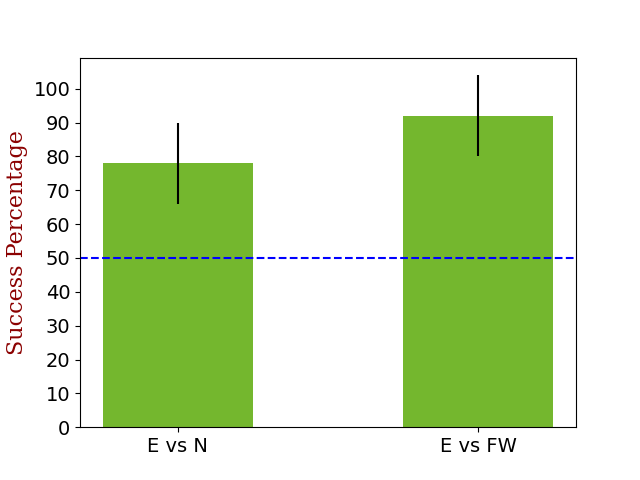
\includegraphics[width=0.98\columnwidth]{images/success_easy_HL.png}\\
	\vspace{-0.7cm}
	\caption{Success percentage in agent superiority identification task for HIGHLIGHTS summaries of agents with high-varying performance}
	\label{fig: HL easy vote}
	\vspace{-0.2cm}
\end{figure}


\section{Summary Sensitivity to Trajectory Horizon}
%%%% summary sensitivity to h
When choosing the trajectory horizon value ($h$), several considerations were kept in mind.
Intuitively, the further an agent is from the disagreement state, the less direct influence that
state has over the agent's current predicament; on the other hand, too low of a value may not
showcase enough of the divergence. In addition, displaying long trajectories in the user study may
lead to loss of participants' interest, while short trajectories can cause the disagreement to be
easily missed. To test the sensitivity of our algorithm to variations in $h$ we observed the top
trajectories obtained for varying values, in the Frogger domain, and noted the shared trajectories between them.
Figure \ref{fig: h_sensitivity} provides evidence that although the sensitivity exists, a
significant proportion of the trajectories stays unhindered even when doubling the value. We note
here that additional constraints that can explain the reduction in shared trajectories include
termination of the simulation and $overlapLim$.

\begin{figure}[ht]
	\centering
    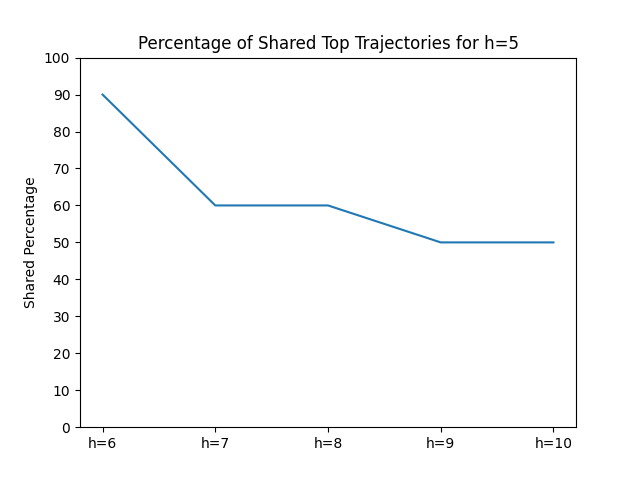
\includegraphics[width=0.98\columnwidth]{images/h_sensitivity.png}\\
	\caption{\disalg~ algorithm sensitivity to horizon parameter $h$}
	\label{fig: h_sensitivity}
	% \vspace{-0.4cm}
\end{figure}

\section{Summary Explanation Satisfaction Questions}
In each experiment participants were asked to rate the following explanation satisfaction statements on a 7-point Likert scale (0 - Strongly disagree to 6 - Strongly agree) for
the summary method they have just witnessed:
\begin{itemize}
	\item From watching the [\emph{method}] videos of the AI agents, I understood which agent is better. 
	\item The [\emph{method}] videos showing the AI agents play contain sufficient detail for deciding which agent is better. 
	\item The [\emph{method}] videos showing the AI agents play contain irrelevant details.
	\item The [\emph{method}] videos showing the AI agents play were useful for the task. 
	\item The specific scenarios shown in the [\emph{method}] videos were useful for the task. 
\end{itemize}
The questionnaire also included an attention check for detecting negligent participants.
Participants who did not answer this question correctly were not included in the analysis.

Explanation satisfaction of participants shown \disalg~ summaries was similar to that of participants shown HIGHLIGHTS summaries. Participants’ distributions of scores for the explanation satisfaction were not statistically significant $(p_{exp\#1} = 0.17, p_{exp\#2} = 0.61)$.

\begin{figure}[ht]
	\centering
    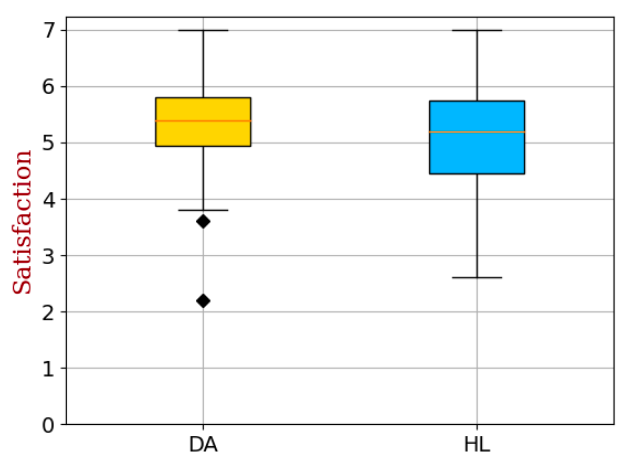
\includegraphics[width=0.98\columnwidth]{images/sat.png}\\
	\caption{\textbf{Frogger:} Participants' Overall Summary Method Satisfaction}
	\label{fig: pref}
\end{figure}

\begin{figure}[ht]
	\centering
    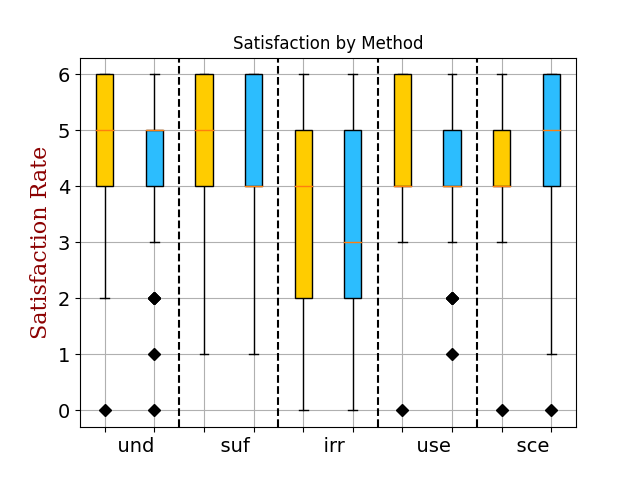
\includegraphics[width=0.98\columnwidth]{images/Satisfaction.png}\\
	\caption{\textbf{Highway:} Participants' Summary Method Satisfaction by Question.}
	\label{fig: pref}
\end{figure}


\section{Summary Method Preference Questions}
After completing Exp\#2, participants were asked to state their preferred summary method (HIGHLIGHTS, \disalg~ or ``Both equally'') for the following attributes:
\begin{itemize}
	\item Which video method was more helpful to you in your task?
	\item Which video method was more pleasing to watch?
	\item Which video method contained more irrelevant information?
\end{itemize}
The results of this comparison are displayed in Figure \ref{fig: pref}.

\begin{figure}[ht]
	\centering
    \includegraphics[width=0.98\columnwidth]{images/preference.png}\\
	\caption{Participants' Summary Method Preference}
	\label{fig: pref}
\end{figure}


%%%% Disagreements algorithm pseudo code
% \section{The \disalg~ Algorithm}
% The \disalg~ algorithm pseudo-code is supplied in Algorithm
% \ref{alg:disagreements}. It's parameters are summarized in
% Table \ref{tb:parameters}. \disalg~ takes as input two agents, one which will
% act as the \emph{Leader} $L$, and another as the \emph{Disagreer} $D$. These
% are used to determine the agents' actions, state evaluations and to progress the
% simulation. $k$ is a budget that determines the number of trajectories desired
% in the output summary, and $l$ is the length of each trajectory. Each summary
% trajectory includes states preceding and succeeding the disagreement state. The
% number of subsequent states to include in a trajectory is determined by $h$. In
% addition, $numSim$ represents the number of simulations to collect disagreement
% states from, and $overlapLim$ is the limit on the number of states that can be
% overlapping between trajectories. The algorithm outputs a summary $\mathbb{S}$
% of the agents' most important disagreements, which is a set of trajectories. The
% importance method used for ranking the disagreements, $impMeth$, is supplied as
% input as well.


% \begin{table}[ht]
%     \centering
%     \small
%     \resizebox{0.85\columnwidth}{!}{%
%     \begin{tabular}{|p{2.2cm}|p{6cm}|}
%     \hline
%     \textbf{Parameter} & \textbf{Description (value used in experiments)}
%     \\
%     \hline
%     $k$                & Summary budget, i.e., number of trajectories (5) \\
%     \hline
%     $l$                & Length of each trajectory (10)
%     \\
%     \hline
%     $h$                 & Number of states following $s$ to include in the
%     trajectory (5)      \\
%     \hline
%     $numSim$           & The number of simulations (episodes) run by the
%     \disalg~ algorithm (10)                      \\
%     \hline
%     $overlapLim$           & Maximal number of shared states allowed between two
%     trajectories in the summary (3) \\
%     \hline
%     $impMeth$          & Importance method used for evaluating disagreements
%     (\emph{Last State}) \\
%     \hline
%     \end{tabular}}
%     \caption{The \disalg~ algorithm parameters. Values in parentheses were used in the experiments.}
%     \label{tb:parameters}
% \end{table}
% \ya{add parameters values for highway}


% %%% explaining the algorithm
% \emph{The Algorithm.} First, three lists are initialized for the Leader traces,
% disagreement states and Disagreer trajectories (lines 4--6). Then, we run
% simulations of the agents (lines 7--27) where in each simulation we collect all
% states seen by the Leader during the execution (line 24), disagreement states
% (line 13), and the Disagreer trajectories (lines 14--19). Each step of the
% simulation, both agents are queried for their choice of next action (lines
% 10--11), if they do not agree on the action --- a disagreement state is added
% (line 13) and a disagreement trajectory is created (lines 14--19), after which
% the simulation is restored to the last disagreement state (line 21). After all
% simulations are completed, all disagreement trajectories (coupled pairs of
% Leader and Disagreer trajectories) are obtained (line 28) and the most
% important ones are passed as output (line 29).   

% \begin{algorithm}[tb]
%     \caption{The \disalg~ algorithm. }
%     \label{alg:disagreements}
% \begin{algorithmic}[1]
%     %\vspace{-0.2cm} \SetAlFnt{\small\sf} \DontPrintSemicolon % Some LaTeX
%     % compilers require you to use \dontprintsemicolon instead
%     \STATE {\bfseries Input:} $\pi_L,\pi_D, k, l, h,$ \STATE $overlapLim,
%     numSim, impMeth$ \STATE {\bfseries Output:} $\mathbb{S}$ \STATE $L_{Tr}
%     \leftarrow$ empty list \textit{\;\;\;\#Leader traces} \STATE $\mathbb{D}
%     \leftarrow$ empty list \textit{\;\;\;\#Disagreement states} \STATE $D_T
%     \leftarrow$ empty list \textit{\;\;\;\#Disagreer trajectories}  \FOR
%     {$i=1$ {\bfseries to} $numSim$} \STATE $sim, s = InitializeSimulation()$
%     \WHILE {$(!sim^{\pi_L}.ended())$} \STATE $a^{\pi_L} \leftarrow
%     sim.getAction(\pi_L(s))$ \STATE $a^{\pi_D} \leftarrow
%     sim.getAction(\pi_D(s))$ \IF{$a^{\pi_L} != a^{\pi_D}$} \STATE
%     $\mathbb{D}.add(s)$ \STATE $d_t \leftarrow$ empty list
%     \textit{\;\;\;\#Disagreer trajectory} \FOR{$i=1$ {\bfseries to} $h$}
%     \STATE $s^{\pi_D} \leftarrow sim.advanceState(\pi_D)$ \STATE $a^{\pi_D}
%     \leftarrow sim.getAction(\pi_D(s))$ \STATE $d_t.add(s)$ \ENDFOR \STATE
%     $D_T.add(d_t)$ \STATE $sim, s = reloadSimulation(D_s[-1])$ \ENDIF \STATE $s
%     \leftarrow sim.advanceState(\pi_L)$ \STATE $L_{traces}.add(s)$ \ENDWHILE
%     \STATE $runs = runs+1$ \ENDFOR \STATE $DA_T \leftarrow
%     disagreementTrajPairs(\mathbb{D},L_{Tr}, D_T, l, h)$ \STATE $\mathbb{S}
%     \leftarrow topImpTraj(DA_T, k, overlapLim, impMeth)$
%     \end{algorithmic}
% \end{algorithm}


\section{Trajectory Importance Methods}
We report here additional trajectory importance methods tested in our work which
were abandoned in favor of the last-sate method which provided in our opinion
the best results. Let us denote the value of a trajectory as
$V({t}_{h}^{\pi}(s))$. 
\begin{itemize}
    \item \textbf{Sum:} 
    $V({t}_{h}^{\pi}(s)) = \sum_i V(s_{+i})$
    \item \textbf{Average:} 
    $V({t}_{h}^{\pi}(s)) = \frac{1}{h} \cdot \sum_i V(s_{+i})$
    \item \textbf{Max-Min:} 
    $V({t}_{h}^{\pi}(s)) = \max_i V(s_{+i}) -  \min_i V(s_{+i})$
    \item \textbf{Max-Avg:}
    $V({t}_{h}^{\pi}(s)) = \max_i V(s_{+i}) - \frac{1}{h} \cdot \sum_i
    V(s_{+i})$
    \item \textbf{Sum Delta:}
    $V({t}_{h}^{\pi}(s)) =  \sum^{h-1}_i \big (V(s_{+i}) - V(s_{+i+1}) \big) $ 
 
\end{itemize}
The above methods calculate $V(t)$ which is then used for calculating the
trajectory importance in the following manner:
$ Im({t}_{h}^{\pi_{L}}(s),{t}_{h}^{\pi_{D}}(s)) = 
|V(t_{h}^{\pi_L}(s)) - V(t_{h}^{\pi_D}(s))| $

\section{Last-State Importance Metrics}
The chosen metric for disagreement importance:
\begin{align}
    Im({t}_{h}^{\pi_{L}}(s),{t}_{h}^{\pi_{D}}(s)) = 
    |V(s^{\pi_L}_{+h}) - V(s^{\pi_D}_{+h})|
\end{align}
identifies trajectories where the agents (while possibly prioritizing alternative outcomes) agree that
one of them has reached a poor state while the other a desirable one. The reason it was chosen was to provides a shared
ground truth regarding the states the agents arrive at.

An additional metric which was tested was the summation of the last state values instead of the subtraction:
\begin{align}
    Im({t}_{h}^{\pi_{L}}(s),{t}_{h}^{\pi_{D}}(s)) = 
    |V(s^{\pi_L}_{+h}) + V(s^{\pi_D}_{+h})|
\end{align}

This metric achieves a higher score the more the agents are in disagreement regarding the values of the arrived last states. 
While optimizing for disagreement, this method fails to convey any grounded information regarding which agent outperforms the other. 

\section{Experiment Survey, Summary Videos and Code}
A PDF file with the principal sections of the experiment surveys, summary videos and the
code used for DISAGREEMENTS and HIGHLIGHTS are provided in the supplementary
files. 
% Provided in supplementary material.



